% GNUPLOT: LaTeX picture with Postscript
\begingroup
  \makeatletter
  \providecommand\color[2][]{%
    \GenericError{(gnuplot) \space\space\space\@spaces}{%
      Package color not loaded in conjunction with
      terminal option `colourtext'%
    }{See the gnuplot documentation for explanation.%
    }{Either use 'blacktext' in gnuplot or load the package
      color.sty in LaTeX.}%
    \renewcommand\color[2][]{}%
  }%
  \providecommand\includegraphics[2][]{%
    \GenericError{(gnuplot) \space\space\space\@spaces}{%
      Package graphicx or graphics not loaded%
    }{See the gnuplot documentation for explanation.%
    }{The gnuplot epslatex terminal needs graphicx.sty or graphics.sty.}%
    \renewcommand\includegraphics[2][]{}%
  }%
  \providecommand\rotatebox[2]{#2}%
  \@ifundefined{ifGPcolor}{%
    \newif\ifGPcolor
    \GPcolorfalse
  }{}%
  \@ifundefined{ifGPblacktext}{%
    \newif\ifGPblacktext
    \GPblacktexttrue
  }{}%
  % define a \g@addto@macro without @ in the name:
  \let\gplgaddtomacro\g@addto@macro
  % define empty templates for all commands taking text:
  \gdef\gplbacktext{}%
  \gdef\gplfronttext{}%
  \makeatother
  \ifGPblacktext
    % no textcolor at all
    \def\colorrgb#1{}%
    \def\colorgray#1{}%
  \else
    % gray or color?
    \ifGPcolor
      \def\colorrgb#1{\color[rgb]{#1}}%
      \def\colorgray#1{\color[gray]{#1}}%
      \expandafter\def\csname LTw\endcsname{\color{white}}%
      \expandafter\def\csname LTb\endcsname{\color{black}}%
      \expandafter\def\csname LTa\endcsname{\color{black}}%
      \expandafter\def\csname LT0\endcsname{\color[rgb]{1,0,0}}%
      \expandafter\def\csname LT1\endcsname{\color[rgb]{0,1,0}}%
      \expandafter\def\csname LT2\endcsname{\color[rgb]{0,0,1}}%
      \expandafter\def\csname LT3\endcsname{\color[rgb]{1,0,1}}%
      \expandafter\def\csname LT4\endcsname{\color[rgb]{0,1,1}}%
      \expandafter\def\csname LT5\endcsname{\color[rgb]{1,1,0}}%
      \expandafter\def\csname LT6\endcsname{\color[rgb]{0,0,0}}%
      \expandafter\def\csname LT7\endcsname{\color[rgb]{1,0.3,0}}%
      \expandafter\def\csname LT8\endcsname{\color[rgb]{0.5,0.5,0.5}}%
    \else
      % gray
      \def\colorrgb#1{\color{black}}%
      \def\colorgray#1{\color[gray]{#1}}%
      \expandafter\def\csname LTw\endcsname{\color{white}}%
      \expandafter\def\csname LTb\endcsname{\color{black}}%
      \expandafter\def\csname LTa\endcsname{\color{black}}%
      \expandafter\def\csname LT0\endcsname{\color{black}}%
      \expandafter\def\csname LT1\endcsname{\color{black}}%
      \expandafter\def\csname LT2\endcsname{\color{black}}%
      \expandafter\def\csname LT3\endcsname{\color{black}}%
      \expandafter\def\csname LT4\endcsname{\color{black}}%
      \expandafter\def\csname LT5\endcsname{\color{black}}%
      \expandafter\def\csname LT6\endcsname{\color{black}}%
      \expandafter\def\csname LT7\endcsname{\color{black}}%
      \expandafter\def\csname LT8\endcsname{\color{black}}%
    \fi
  \fi
    \setlength{\unitlength}{0.0500bp}%
    \ifx\gptboxheight\undefined%
      \newlength{\gptboxheight}%
      \newlength{\gptboxwidth}%
      \newsavebox{\gptboxtext}%
    \fi%
    \setlength{\fboxrule}{0.5pt}%
    \setlength{\fboxsep}{1pt}%
\begin{picture}(5668.00,3968.00)%
    \gplgaddtomacro\gplbacktext{%
      \csname LTb\endcsname%%
      \put(434,3322){\makebox(0,0)[r]{\strut{}$0$}}%
      \csname LTb\endcsname%%
      \put(434,3594){\makebox(0,0)[r]{\strut{}$0.9$}}%
      \csname LTb\endcsname%%
      \put(434,3866){\makebox(0,0)[r]{\strut{}$1.8$}}%
      \csname LTb\endcsname%%
      \put(566,3041){\makebox(0,0){\strut{}}}%
      \csname LTb\endcsname%%
      \put(1168,3041){\makebox(0,0){\strut{}}}%
      \csname LTb\endcsname%%
      \put(1770,3041){\makebox(0,0){\strut{}}}%
      \csname LTb\endcsname%%
      \put(2372,3041){\makebox(0,0){\strut{}}}%
      \csname LTb\endcsname%%
      \put(2975,3041){\makebox(0,0){\strut{}}}%
      \csname LTb\endcsname%%
      \put(3577,3041){\makebox(0,0){\strut{}}}%
      \csname LTb\endcsname%%
      \put(4179,3041){\makebox(0,0){\strut{}}}%
      \csname LTb\endcsname%%
      \put(4781,3041){\makebox(0,0){\strut{}}}%
      \csname LTb\endcsname%%
      \put(5383,3041){\makebox(0,0){\strut{}}}%
    }%
    \gplgaddtomacro\gplfronttext{%
      \csname LTb\endcsname%%
      \put(-171,3594){\rotatebox{-270}{\makebox(0,0){\strut{}$C_{out}$}}}%
      \put(2974,2975){\makebox(0,0){\strut{}}}%
    }%
    \gplgaddtomacro\gplbacktext{%
      \csname LTb\endcsname%%
      \put(434,2655){\makebox(0,0)[r]{\strut{}$0$}}%
      \csname LTb\endcsname%%
      \put(434,2928){\makebox(0,0)[r]{\strut{}$0.9$}}%
      \csname LTb\endcsname%%
      \put(434,3200){\makebox(0,0)[r]{\strut{}$1.8$}}%
      \csname LTb\endcsname%%
      \put(566,2375){\makebox(0,0){\strut{}}}%
      \csname LTb\endcsname%%
      \put(1168,2375){\makebox(0,0){\strut{}}}%
      \csname LTb\endcsname%%
      \put(1770,2375){\makebox(0,0){\strut{}}}%
      \csname LTb\endcsname%%
      \put(2372,2375){\makebox(0,0){\strut{}}}%
      \csname LTb\endcsname%%
      \put(2975,2375){\makebox(0,0){\strut{}}}%
      \csname LTb\endcsname%%
      \put(3577,2375){\makebox(0,0){\strut{}}}%
      \csname LTb\endcsname%%
      \put(4179,2375){\makebox(0,0){\strut{}}}%
      \csname LTb\endcsname%%
      \put(4781,2375){\makebox(0,0){\strut{}}}%
      \csname LTb\endcsname%%
      \put(5383,2375){\makebox(0,0){\strut{}}}%
    }%
    \gplgaddtomacro\gplfronttext{%
      \csname LTb\endcsname%%
      \put(-171,2927){\rotatebox{-270}{\makebox(0,0){\strut{}$R_4$}}}%
      \put(2974,2309){\makebox(0,0){\strut{}}}%
    }%
    \gplgaddtomacro\gplbacktext{%
      \csname LTb\endcsname%%
      \put(434,1989){\makebox(0,0)[r]{\strut{}$0$}}%
      \csname LTb\endcsname%%
      \put(434,2261){\makebox(0,0)[r]{\strut{}$0.9$}}%
      \csname LTb\endcsname%%
      \put(434,2533){\makebox(0,0)[r]{\strut{}$1.8$}}%
      \csname LTb\endcsname%%
      \put(566,1708){\makebox(0,0){\strut{}}}%
      \csname LTb\endcsname%%
      \put(1168,1708){\makebox(0,0){\strut{}}}%
      \csname LTb\endcsname%%
      \put(1770,1708){\makebox(0,0){\strut{}}}%
      \csname LTb\endcsname%%
      \put(2372,1708){\makebox(0,0){\strut{}}}%
      \csname LTb\endcsname%%
      \put(2975,1708){\makebox(0,0){\strut{}}}%
      \csname LTb\endcsname%%
      \put(3577,1708){\makebox(0,0){\strut{}}}%
      \csname LTb\endcsname%%
      \put(4179,1708){\makebox(0,0){\strut{}}}%
      \csname LTb\endcsname%%
      \put(4781,1708){\makebox(0,0){\strut{}}}%
      \csname LTb\endcsname%%
      \put(5383,1708){\makebox(0,0){\strut{}}}%
    }%
    \gplgaddtomacro\gplfronttext{%
      \csname LTb\endcsname%%
      \put(-171,2261){\rotatebox{-270}{\makebox(0,0){\strut{}$R_3$}}}%
      \put(2974,1642){\makebox(0,0){\strut{}}}%
    }%
    \gplgaddtomacro\gplbacktext{%
      \csname LTb\endcsname%%
      \put(434,1322){\makebox(0,0)[r]{\strut{}$0$}}%
      \csname LTb\endcsname%%
      \put(434,1594){\makebox(0,0)[r]{\strut{}$0.9$}}%
      \csname LTb\endcsname%%
      \put(434,1866){\makebox(0,0)[r]{\strut{}$1.8$}}%
      \csname LTb\endcsname%%
      \put(566,1041){\makebox(0,0){\strut{}}}%
      \csname LTb\endcsname%%
      \put(1168,1041){\makebox(0,0){\strut{}}}%
      \csname LTb\endcsname%%
      \put(1770,1041){\makebox(0,0){\strut{}}}%
      \csname LTb\endcsname%%
      \put(2372,1041){\makebox(0,0){\strut{}}}%
      \csname LTb\endcsname%%
      \put(2975,1041){\makebox(0,0){\strut{}}}%
      \csname LTb\endcsname%%
      \put(3577,1041){\makebox(0,0){\strut{}}}%
      \csname LTb\endcsname%%
      \put(4179,1041){\makebox(0,0){\strut{}}}%
      \csname LTb\endcsname%%
      \put(4781,1041){\makebox(0,0){\strut{}}}%
      \csname LTb\endcsname%%
      \put(5383,1041){\makebox(0,0){\strut{}}}%
    }%
    \gplgaddtomacro\gplfronttext{%
      \csname LTb\endcsname%%
      \put(-171,1594){\rotatebox{-270}{\makebox(0,0){\strut{}$R_2$}}}%
      \put(2974,975){\makebox(0,0){\strut{}}}%
    }%
    \gplgaddtomacro\gplbacktext{%
      \csname LTb\endcsname%%
      \put(434,656){\makebox(0,0)[r]{\strut{}$0$}}%
      \csname LTb\endcsname%%
      \put(434,928){\makebox(0,0)[r]{\strut{}$0.9$}}%
      \csname LTb\endcsname%%
      \put(434,1200){\makebox(0,0)[r]{\strut{}$1.8$}}%
      \csname LTb\endcsname%%
      \put(566,375){\makebox(0,0){\strut{}0}}%
      \csname LTb\endcsname%%
      \put(1168,375){\makebox(0,0){\strut{}100}}%
      \csname LTb\endcsname%%
      \put(1770,375){\makebox(0,0){\strut{}200}}%
      \csname LTb\endcsname%%
      \put(2372,375){\makebox(0,0){\strut{}300}}%
      \csname LTb\endcsname%%
      \put(2975,375){\makebox(0,0){\strut{}400}}%
      \csname LTb\endcsname%%
      \put(3577,375){\makebox(0,0){\strut{}500}}%
      \csname LTb\endcsname%%
      \put(4179,375){\makebox(0,0){\strut{}600}}%
      \csname LTb\endcsname%%
      \put(4781,375){\makebox(0,0){\strut{}700}}%
      \csname LTb\endcsname%%
      \put(5383,375){\makebox(0,0){\strut{}800}}%
    }%
    \gplgaddtomacro\gplfronttext{%
      \csname LTb\endcsname%%
      \put(-171,928){\rotatebox{-270}{\makebox(0,0){\strut{}$R_1$}}}%
      \put(2974,45){\makebox(0,0){\strut{}tempo $[ns]$}}%
    }%
    \gplbacktext
    \put(0,0){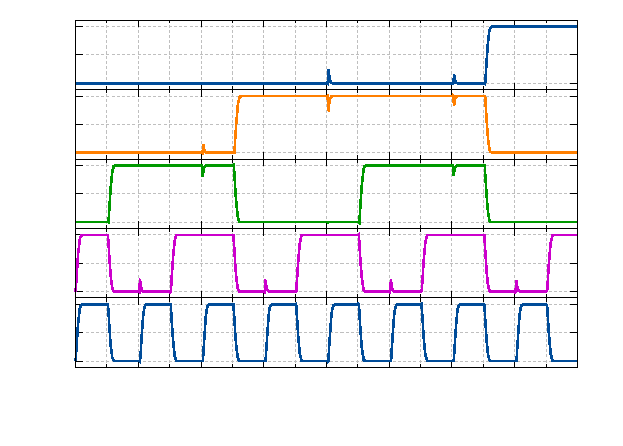
\includegraphics[width={283.40bp},height={198.40bp}]{Immagini/4bit-adder-sim}}%
    \gplfronttext
  \end{picture}%
\endgroup

